\documentclass[10pt,journal]{IEEEtran}
%\IEEEoverridecommandlockouts

\usepackage[spanish,es-tabla]{babel} % Idioma español con tablas
\usepackage[spanish]{babel}
\usepackage[table,xcdraw]{xcolor} % Para pintar tablas
\usepackage{url} % Para colocar URL
\usepackage{amsmath,amssymb,amsfonts}
\usepackage{graphicx}
\usepackage{textcomp}
\usepackage{xcolor}
\usepackage{float} % Para var H, figure

\usepackage[square,numbers]{natbib}
\bibliographystyle{abbrvnat}

\renewcommand{\baselinestretch}{1.5}     %interlineado

\title{Ideas de Investigaciones en Informática o Ciencias de la Computación}

\author{
\IEEEauthorblockN{{\Large Angely Mendez Cruz}} \\
\vspace{2mm}
\IEEEauthorblockA{\textit{Metodología de la Investigación Científica} \\
\textit{Escuela de Informática} \\
\textit{Facultad de Ciencias Físicas y Matemáticas} \\
\textit{Universidad Nacional de Trujillo, \\ Perú }
\\ \vspace{1mm}
t052701020@unitru.edu.pe}}

\begin{document}
\renewcommand{\IEEEkeywordsname}{{\bfseries Palabras claves:}} % Colocar Keywords en Spanish

\maketitle

    \begin{abstract}
    En este trabajo de investigación se brinda información respecto a 5 ideas de investigación, las cuales son: Interacción Humano-computadora (IHC), Sistema de Hardware, Interfaz cerebro-computadora extendida (CCI), Internet de las Cosas y Computación en la Nube, y el Procesamiento Paralelo de imágenes, las que posteriormente se convirtieron en temas específicos cuya finalidad son aplicaciones de la informática en la realidad; donde se ha tenido en cuenta conocimientos sobre ciencias de la computación, la tecnología existente y la propuesta e incluso ejecución de nuevas tecnologías propias, algoritmos eficientes e investigaciones externas.
    \end{abstract}
    
    \begin{IEEEkeywords}
    Ideas, investigación, informática, ciencias de la computación.
    \end{IEEEkeywords}
    
    \section{\textbf{Introducción}}
    
    En la actualidad y ante el planteamiento de resolver problemáticas, las ideas son el punto de partida para realizar una investigación, donde constituyen el primer acercamiento a la realidad que habrá de investigarse. Para muchos pareciera que esta etapa es fácil, y lo es, siempre y cuando el investigador tenga experiencia en el campo investigativo y amplios conocimientos en su área disciplinaria
    
    Como todo parte de una idea esta nos debe interesar, atraer y resultar útil para aplicar. Dentro de la informática o Ciencias de la Computación existen diversos temas en los que investigar, antes se debe tener conocimiento respecto a la idea de la investigación, debemos ser capaces de usar la observación y el análisis de la realidad.

    Algunos de los medios de difusión sobre las ideas e investigaciones son las revistas, artículos e internet, tal como el presente artículo que expone diversas ideas dentro de la informática, sus aplicaciones fueron pensadas analizando la realidad, para posteriormente ser aplicables en beneficio del medio ambiente, las personas y salud. 

    \section{\textbf{Ideas de Investigaciones en Informática o Ciencias de la Computación}}
    \subsection{\underline{\textbf{Interacción Humano-computadora (IHC)}}}
    Según Adobe Xd Ideas \citep{HumanCom81}, define a la interacción humano-computadora (IHC) como el campo de diseño que se enfoca en las interfaces entre las personas y las computadoras. El cual tiene un impacto directo en la eficiencia de la interacción entre las dos partes.
    
    IHC surgió en la década de 1980 con la popularización de la informática personal. Las computadoras ya no se construían solo para expertos, y el objetivo de IHC era hacer que todas las interacciones con las computadoras fueran fáciles y eficientes para amplios grupos de usuarios con diferentes niveles de habilidad. A continuación se una investigación respecto a esta idea:
    \begin{itemize}
        \item Con el fin de mejorar la confiabilidad, movilidad y facilidad de uso de la técnica de seguimiento ocular en el diálogo usuario-computadora, en la investigación titulada \textit{Sistema de control basado en el seguimiento ocular para la interacción natural entre humanos y computadoras} \citep{zhang2017eye}, se propone un novedoso sistema de control ocular que integra funciones de mouse y teclado. 
        El movimiento de los ojos se considera como un medio fundamental de entrada en tiempo real para la comunicación entre humanos y computadoras, lo cual es especialmente importante para las personas con discapacidades físicas. El sistema mencionado se enfoca en proporcionar un modo interactivo simple y conveniente usando solo el ojo del usuario. El flujo de uso del sistema está diseñado para seguir perfectamente los hábitos naturales humanos, obsérvese en la Figura ~\ref{f1}. Además, se propone un módulo de lupa que permite la operación precisa. 
        \begin{figure}[H]
        \begin{center}
        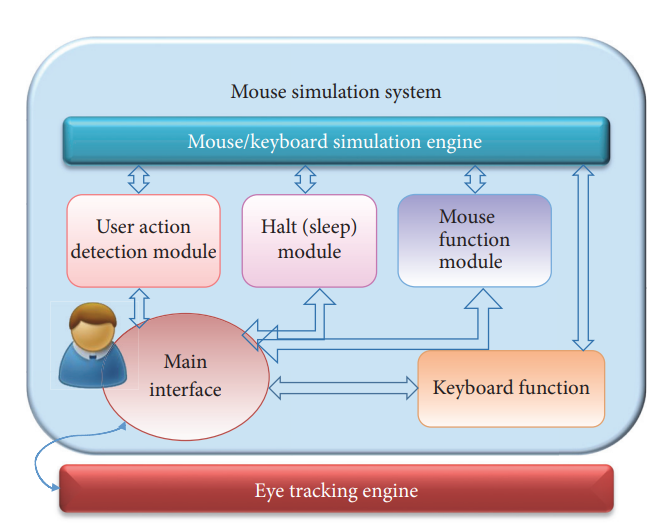
\includegraphics[width=7.5cm, height=4.8cm]{figuras/eyes.PNG}
        \caption{La arquitectura del sistema.}
        \label{f1} 
        \end{center}
        \end{figure}
        
        En el experimento, se realizaron dos tareas interactivas con diferente dificultad (búsqueda de artículos y navegación web multimedia) para comparar la herramienta de control ocular propuesta con un sistema existente.
        \\ Las medidas del Modelo de aceptación de tecnología (TAM) se utilizan para evaluar la eficacia percibida en el sistema, demostrando que el sistema es muy efectivo en cuanto a usabilidad y diseño de interfaz.
        
    \end{itemize}
    
    \subsection{\underline{\textbf{Sistema de Hardware}}}
    Dentro de la informática, un sistema de hardware es el conjunto de todas las partes físicas, tangibles (que se pueden tocar), mecánicas, eléctricas, electrónicas, electromecánicos.

    A lo largo de la historia de los equipos de cómputo el hardware cumple lo más fundamental para que este funcione. Y ha tenido que evolucionar rápidamente para obtener un mayor rendimiento y poder realizar el mayor número de procesos en el menor tiempo posible.
    
    Una investigación sobre sistema de Hardware es el siguiente:
    \begin{itemize}
    \item  \textit{Investigación de Sistema de Control para UAV de Protección de Plantas Basado en Pixhawk} \citep{YANG2020371},este trabajo propuso el sistema de control de UAV fitosanitario basado en el controlador de vuelo Pixhawk, donde el sistema consta de dos subsistemas: sistema de control de vuelo y sistema de aspersión. Se  adoptó el firmware basado en PX4 para lograr el control de vuelo Pixhawk.
    
    El sistema de hardware de control de UAV de protección de plantas se muestra en la Figura ~\ref{f2}, incluye el intercambio de datos entre el sistema de control de vuelo y el sistema de pulverización a través del puerto serie. 
    \\ El protocolo de comunicación se analizo en detalle y se realizó el control de comunicación entre el controlador de vuelo y el controlador de pulverización por puerto serie. La parte del software ha sido diseñada para la tarea de decodificación del control remoto y la tarea de rociado en el sistema de control de vuelo y la tarea de rociado en el sistema de rociado.
    \begin{figure}[H]
        \begin{center}
        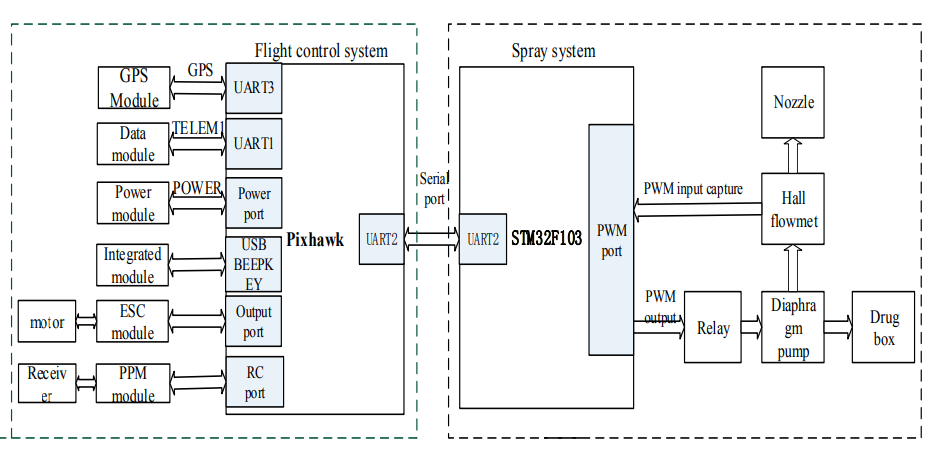
\includegraphics[width=9cm, height=4cm]{figuras/hardware.PNG}
        \caption{Diagrama del Sistema de Hardware.}
        \label{f2} 
        \end{center}
    \end{figure}
    
     Finalmente, se tomó el UAV de protección de plantas como objeto, la comunicación entre el sistema de control de vuelo y el sistema de rociado se realizó para completar la función de rociado con éxito.
    \end{itemize}
    
    \subsection{\underline{\textbf{Interfaz cerebro-computadora extendida (CCI)}}}
    Según la definición que establece \citep{trofimov2011brain} se entiende por CCI, sus siglas en inglés BCI (brain-computer interface), es un sistema que decodifica la actividad neuronal del usuario (ej., señales eléctricas, campos magnéticos, flujo sanguíneo), con la finalidad de controlar dispositivos (principalmente prótesis o sillas de ruedas) que permitan devolverle la independencia a personas que han perdido.
    
    Por lo expuesto anteriormente a continuación se menciona una investigación respecto a ello.
    
    \begin{itemize}
    \item  \textit{El sistema de control basado en CCI extendido para una silla de ruedas robótica} \citep{VOZNENKO2018522},
    En la mayoría de los casos, el movimiento de las sillas de ruedas lo controlan personas discapacitadas mediante un joystick o un acompañante. Los pacientes con discapacidad significativa necesitan métodos de control alternativos sin utilizar el joystick de la silla de ruedas porque es indeseable o imposible para estos pacientes. En este artículo, se presentó la implementación de una silla de ruedas robótica basada en una silla de ruedas eléctrica controlada no por el joystick sino por la computadora a bordo que recibe y procesa datos de la interfaz cerebro-computadora extendida (CCI extendida), como se muestra en la Figura ~\ref{f36}. 
    
    \begin{figure}[H]
        \begin{center}
        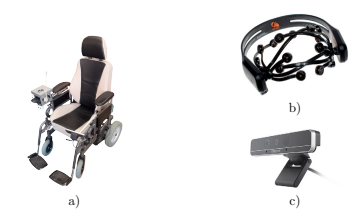
\includegraphics[width=6cm, height=4cm]{figuras/silla2.PNG}
        \caption{a)La “silla” b)BCI Epoc Emotiv c)Intel RealSense}
        \label{f36} 
        \end{center}
    \end{figure}
    
    Bajo este término se entendió el sistema de control complejo robótico con canales de control alternativos independientes simultáneos. En esta versión de silla de ruedas robótica, el CCI funciona con canales de control de voz y gestos.
    
    Este proyecto de la “silla” ha recibido una cobertura bastante amplia en los medios de comunicación rusos y extranjeros, ver en la Figura ~\ref{f3}, como la prensa de España y países de habla hispana, por ejemplo en El Diario de Hoy, El Universal y en China (Science and Technology Daily.
    
    \begin{figure}[H]
        \begin{center}
        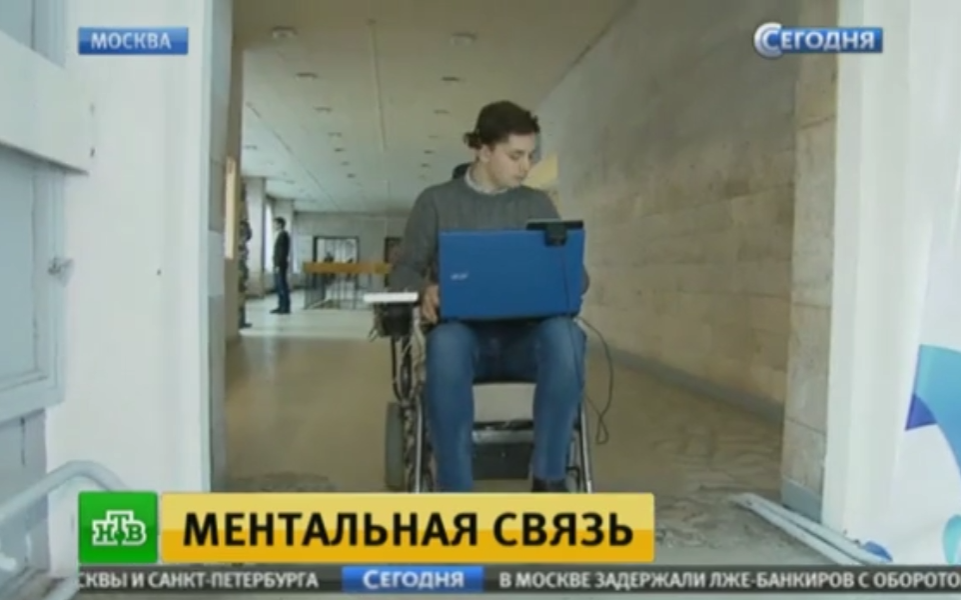
\includegraphics[width=6.5cm, height=4cm]{figuras/silla.PNG}
        \caption{Sistema de control en los medios de comunicación.}
        \label{f3} 
        \end{center}
    \end{figure}
    \end{itemize}
    
    \subsection{\underline{\textbf{Internet de las Cosas y Computación en la Nube}}}
    Según se entiende la Internet de las cosas (IoT) describe la red de objetos físicos ('cosas') que llevan incorporados sensores, software y otras tecnologías con el fin de conectarse e intercambiar datos con otros dispositivos y sistemas a través de Internet. Por otro lado, la computación en la nube es un modelo de entrega donde el almacenamiento, los servidores, las aplicaciones y otros elementos se entregan por Internet. 
    
    A continuación se una investigación respecto a esta idea:
    
    \begin{itemize}
    \item  \textit{Sistema de Prealarma Basado en Monitoreo en Tiempo Real y Simulación Numérica Utilizando Internet de las Cosas y Computación en la Nube para Presa de Relaves en Minas} \citep{dong2017pre}. La presa de relaves, una instalación necesaria para mantener el funcionamiento normal de las empresas mineras, es una fuente peligrosa de flujo de escombros causado por el hombre con un alto potencial de energía. La prealarma en tiempo real para la inestabilidad de la presa de relaves es vital para garantizar la minería normal y la seguridad de las vidas humanas y las propiedades.
    
    Basado en Internet de las cosas y redes inalámbricas, el sistema de información clave y múltiple de la presa de relaves se construye utilizando los datos de los sensores, que incluyen los índices de estabilidad como la línea freática, el nivel del agua del embalse, la deformación interna y externa de la presa de relaves, ver en la Figura ~\ref{f56}. La plataforma en la nube se aplica para predecir el estado futuro de la línea freática en función de los datos de monitoreo en tiempo real, donde se puede obtener la ecuación de la línea freática. El modelo de simulación numérica se establece considerando la ecuación predicha de la línea freática, los parámetros del estado de equilibrio límite, el nivel del agua del embalse y la precipitación. Luego, el factor de seguridad, la confiabilidad aleatoria y la confiabilidad no probabilística de intervalo se puede resolver a través de la plataforma en la nube. En combinación con la tendencia de la deformación del monitoreo en tiempo real, así como el factor de seguridad dinámico calculado, la confiabilidad aleatoria y la confiabilidad no probabilística de intervalo, las señales de advertencia estables o peligrosas de la presa de relaves se pueden obtener mediante la prealarma remota en tiempo real. El principal método resuelto para los parámetros clave y el proceso de prealarma se presentaron a través de un estudio de caso.
    
     \begin{figure}[H]
        \begin{center}
        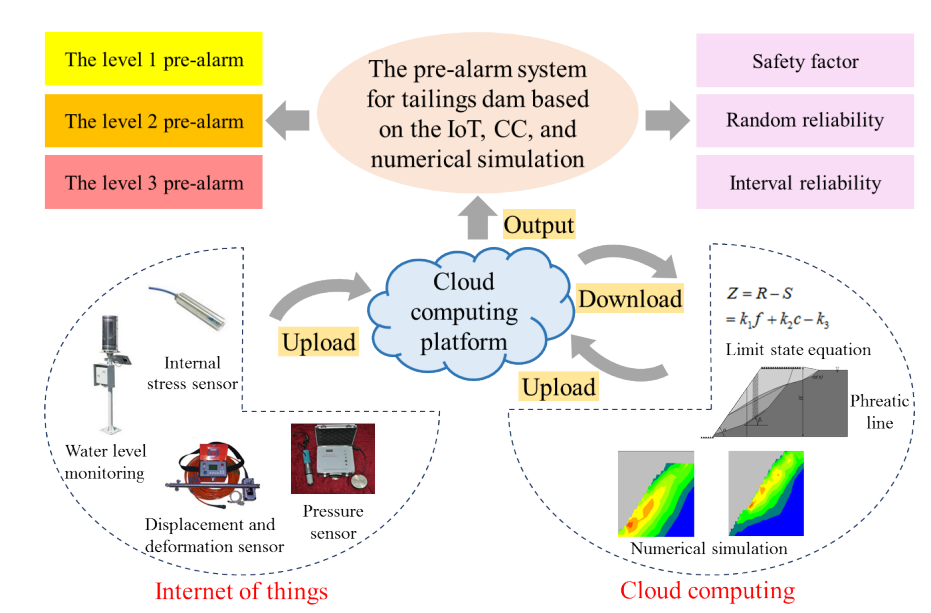
\includegraphics[width=8cm, height=5cm]{figuras/tailing.PNG}
        \caption{Diagrama del Funcionamiento del Sistema de Pre-alarma.}
        \label{f56} 
        \end{center}
    \end{figure}
    \end{itemize}
    
    \subsection{\underline{\textbf{Procesamiento Paralelo de imágenes}}}
    El procesamiento paralelo de imágenes digitales es el conjunto de técnicas que se aplican a las imágenes digitales con el objetivo de mejorar la calidad o facilitar la búsqueda de información, los cuales dichos procesos paralelos en un ordenador se ejecutan y/o procesan a la vez.
    
    EL procesamiento de imágenes tiene como objetivo mejorar el aspecto de las imágenes y hacer más evidentes en ellas ciertos detalles que se desean hacer notar. La imagen puede haber sido generada de muchas maneras, por ejemplo, fotográficamente, o electrónicamente, por medio de monitores de televisión.
    
    Por lo expuesto anteriormente a continuación se menciona una investigación respecto a ello.
    
    \begin{itemize}
    \item  \textit{Procesamiento paralelo de imágenes de video para la detección de sangrado y vendas en operaciones de cirugía laparoscopica} \citep{derwael2015procesamiento}, se presenta una aplicación de procesamiento de imagen para un entorno robotizado destinado a asistir a un médico en operaciones de cirugía laparoscópica. Durante la operación el robot, a través del sistema de visión, deberá detectar cuándo aparece una situación de sangrado dentro de la cavidad abdominal con objeto de ayudar al cirujano a atajar esta situación. El sistema de procesamiento de imágenes se ha ampliado también a la detección de vendas para garantizar que se retiran todas al finalizar la operación.
    
    Con objeto de permitir un procesamiento en tiempo real de las imágenes de vídeo, el sistema desarrollado realiza un procesamiento en paralelo dividiendo las diferentes tareas entre todos los núcleos existentes en el procesador empleando la biblioteca Intel TBB. 
    
    Los resultados obtenidos sobre esta investigación de la aplicación tanto en la detección de sangrado, obsérvese Figura ~\ref{f76} como de vendas son muy satisfactorios.
    
    El algoritmo funciona en tiempo real y tiene unas buenas tasas de detección. No obstante, actualmente se está trabajando para introducir mejoras en la detección de sangre introduciendo umbrales adaptativos para el color. Esto permitirá dotar de mayor fiabilidad al algoritmo cuando existan cambios significativos en la iluminación.

     \begin{figure}[H]
        \begin{center}
        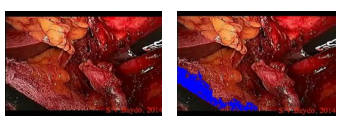
\includegraphics[width=8cm, height=5cm]{figuras/medicc.PNG}
        \caption{Resultados sobre la detección de una venda ensangrentada en una imagen.}
        \label{f76} 
        \end{center}
    \end{figure}
    \end{itemize}
    
    
    \section{\textbf{Conclusiones}}
    Para concluir, las ideas presentadas en esta investigación, que dieron paso a la formación de varios temas, demuestran que las aplicaciones de la informática son diversas y muy útiles en la sociedad, debido a que la tecnología ha crecido de manera tan exponencial en los últimos años por lo que ha habido una demanda cada vez mayor de resolver problemáticas con ayuda de ella, que transformen áreas que van desde la salud de las personas hasta el medio ambiente. Finalmente, las investigaciones en la informática expuestas en este trabajo de recopilación, sirven como antecedentes y base a futuros investigadores a nivel nacional e internacional, que pueden ser usados tanto en el área comercial o académico.
\medskip
\bibliography{Referencia}

\end{document}
